\section{Lessons Learned Perspective}
\subsection{Most Important Issues}
\subsubsection{Evolution and Refactoring}
The main issue we had with the refactoring of the old code was the lack of documentation. 
A large part of the group had no proficiency with neither Python nor Flask, and we were therefore 
forced to invest a lot of time into understanding the system. 
One of the takeaways from this was how difficult it can be to understand and further develop 
old code when there is a lack of documentation. 
This is an important lesson because this situation often takes place in the real world.

To challenge us as a DevOps team, we decided to also evolve the existing functionality further, by adding new features. 
Examples of this are the application's new design and the chat-functionality. 
Although these functionalities were not our main focus area, they still provided 
a useful learning experience in continuous deployment and a training in how to release small features often.

\subsubsection{Maintenance and Operation}

Regarding maintenance and operation, one of the primary issues was that we often had some periods with long downtime. 
For the sake of simplicity, we have narrowed it down to four different major down periods in this report. 
These are marked with blue (from now on referred to as the 'first'), dark blue (from now on referred to as 'second'), 
yellow (from now on referred to as 'third'), and green (from now on referred to as the 'last') in figure 1 below. 

\begin{figure}[h!]
    \centering
    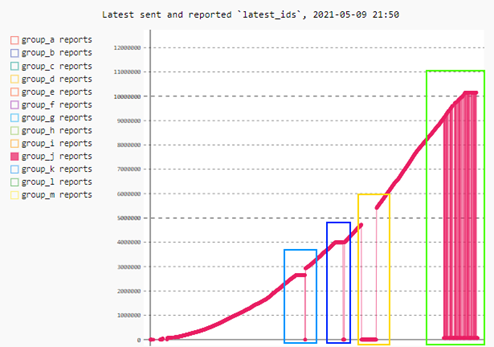
\includegraphics[scale=0.7]{images/downperiodes.png}
    \caption{The graph showing "latest", an integer which is updated for each completed job sent from the simulator, 
    thus keeping track of the current simulation progress. }
\end{figure}
 
All these different downtime periods had different solutions, and we have decided to discuss the two down periods we 
learned the most from: the first down period and the second one. 
The first down period was due to a crash with our database software (PostgreSQL), and in the second down period, 
was due to a simulator-side crash. Although logging helped us out in the last down period, 
we realized too late that the system was down, resulting in a longer period of downtime. 
The major lesson learned from the two down periods was that we should have implemented some sort of alerting 
that would send alerts to all the team members in case of a failure. This was something we started to 
implement in Kibana. Unfortunately, due to the lack of time at the end of the simulation, we did not have time to implement this.

\subsubsection{DevOps way of working}
Throughout the project, we as a group have kept the “three ways” characterizing DevOps in mind: 
flow, feedback, and continual learning and experimentation \cite{devopshandbook}.

\textbf{Principles of Flow}

While working on our system, we tried to limit the work in progress by releasing it, to the production environment as often as possible. 
This enabled us to have a clear idea of what had changed since last time. 
Which also made it easier for us to roll back and immediately locate bugs if the system was to crash.

\textbf{The Principles of Feedback}

With tools to monitor our system, we had constant feedback on how our system was performing. 
This was useful to get to see the problems as they occured, and to quickly act upon them. 
As we attempted to release quickly and efficiently, bugs sometimes slipped through the quality gates in our CI pipelines. 
When bugs did slip through, we as a team gathered to solve them in unity, enabling us to share knowledge and experiences. 
This was different from what we had done in other projects, that did not follow the DevOps principles, where it often was a single person who solved the issue.

\textbf{The Principles of Continual Learning and Experimentation}

On our bi-weekly group meetings, we shared learning points and challenges we had stumbled into, when working individually since the last meeting.
 We have also used the wiki tool and the issue tracker/project-board on Github to document as many issues and changes as possible, 
 as well as making it easy to get an overview of the project's progression.

